\section{Building molecules}

Since BALL is intended for Molecular Modeling, the classes representing atoms,
bonds, and molecules are of central importance. In this first example, we will
construct a water molecule ``by hand'' to illustrate the use of these classes.
Typical applications would read molecular structures from a file. This will be
shown in the second example.

\noindent
To start the construction of a water molecule, we first create an (empty)
\Index{atom}. Atoms are represented by the class \class{Atom}.

\begin{lstlisting}{}
	Atom* oxygen = new Atom;
\end{lstlisting}
	
\noindent
Atoms have a number of attributes. As we created this atom without specifying
any of its properties, these attributes are set to their defaults. The
following table lists the attributes of an atom along with its
\newtermdef{accessors} (methods to access or modify an attribute) and default
values.
\begin{center}
	\begin{tabular}{lllc}
	attribute		&	type				& accessors     						& default\\
	\hline
	name				& String			& setName,getName						& {\tt ""}\\
	element			& Element			& setElement,getElement			& {\tt Element::UNKNOWN}\\
	charge			& float				& setCharge,getCharge				& 0.0\\
	radius			& float				& setRadius,getRadius				& 0.0\\
	type name   & String			& setTypeName,getTypeName		& {\tt ""}\\
	type        & Atom::Type	& setType,getType						& {\tt Atom::INVALID\_TYPE}\\
	position    & Vector3			& setPosition,getPosition		& (0, 0, 0)\\
	velocity    & Vector3			& setVelocity,getVelocity		& (0, 0, 0)\\
	force		    & Vector3			& setForce,getForce					& (0, 0, 0)
	\end{tabular}
\end{center}

\noindent
For example, we can assign the \Index{element} for our new atom:

\begin{lstlisting}{}
	oxygen->setElement(PTE[Element::O]);
\end{lstlisting}

\noindent
The expression {\tt PTE[\class{Element}::O]} returns an instance of class
\class{Element}. It is assigned to our atom using the \method{setElement}
method. We leave our new atom at the default position (0, 0, 0) and create two
new atoms, which will be the still missing hydrogen atoms:

\begin{lstlisting}{}
	Atom* hydrogen1 = new Atom;
	Atom* hydrogen2 = new Atom;
	hydrogen1->setElement(PTE[Element::H]);
	hydrogen2->setElement(PTE[Element::H]);
\end{lstlisting}
	
\noindent
Now we have to assign the correct coordinates to the two hydrogen atoms.  The
method \method{setPosition} takes an instance of \class{Vector3} as an
argument. This class is used to represent coordinates and vectors in
three--dimensional space. An object of type \class{Vector3} can be constructed
from three floating point numbers which represent the x, y, and z coordinates.
Thus, we can assign the coordinates as follows:
 
\begin{lstlisting}{}
 	hydrogen1->setPosition(Vector3(-0.95, 0.00, 0.0));
 	hydrogen2->setPosition(Vector3( 0.25, 0.87, 0.0));
\end{lstlisting}

\noindent

Now, our three atoms are of the right type and at the right positions. However, we
do not yet have a molecule, so let's create one:\\

\begin{lstlisting}{}
	Molecule* water = new Molecule;
\end{lstlisting}

\noindent
Molecules are representd by the \class{Molecule} class. Each instance of this
class may contain an arbitrary number of atoms. Using the \method{insert}
method, we can construct a molecule from our atoms:

\begin{lstlisting}{}
	water->insert(*oxygen);
	water->insert(*hydrogen1);
	water->insert(*hydrogen2);
\end{lstlisting}

\noindent
For a complete water molecule, we still need two \Index{bonds}. This can be
achieved with the method \method{createBond}:
	
\begin{lstlisting}{}
	oxygen->createBond(*hydrogen1);
	oxygen->createBond(*hydrogen2);
\end{lstlisting}

or

\begin{lstlisting}{}
	hydrogen2->createBond(*oxygen);
\end{lstlisting}

\noindent
To verify that everything worked as expected, we might print the number of
atoms in the molecule or the number of bonds for each atom:
	
\begin{lstlisting}{}
	cout << "# of atoms in water: " 
 			 << water->countAtoms() << endl;
	cout << "# of bonds of oxygen: " 
			 << oxygen->countBonds() << endl;
	cout << "# of bonds of hydrogen1: " 
		   << hydrogen1->countBonds() << endl;
	cout << "# of bonds of hydrogen2: " 
			 << hydrogen2->countBonds() << endl;
\end{lstlisting}

\noindent
The method \method{countAtoms} is available for all kernel classes that might
contain atoms and returns the total number of atoms for this object. The
method \method{countBonds} returns the number of bonds the atom shares. An
atom can have at most eight bonds.

We can also verify the bond distances:
\begin{lstlisting}{}
	Vector3 bond_vector = oxygen->getPosition() 
										    - hydrogen1->getPosition();

	cout << "bond distance: " 
			 << bond_vector.getLength() << endl;
\end{lstlisting}
	
\noindent
\method{getPosition} is the complementary method of \method{setPosition}: it
returns the current position of an atom. The return value is again of type
\class{Vector3}. The length of this vector is then returned by the
\method{getLength} method. 

Water molecules rarely occur alone, so we are going to create further water.
All BALL kernel classes are container classes and support \newterm{deep
copying}, \ie when assigned or copy constructed their contents are copied as
well. So, we can easily create a new water molecule:

\begin{lstlisting}{}
	Molecule* water2 = new Molecule(*water);
\end{lstlisting}
	
\noindent
This molecule is an exact copy of our original water molecule. Especially, the
atoms have the same position as in the original. So we want to shift the whole
molecule to another position.  In principle, we could access all atoms in the
copy and add a constant translation vector to their position. However, there
is a simpler way. BALL provides so--called \newterm{processors}. These
processors may be applied to any of the kernel objects and perform an
operation on any objects they encounter. For example the
\class{TranslationProcessor} performs a simple translation on every atom it
finds. The use of the processors is very simple.  All kernel classes define an
\method{apply} method wich takes a processor as an argument. In order to
translate our second water molecule by a certain distance, we first create a
\class{TranslationProcessor}:

\begin{lstlisting}{}
	TranslationProcessor translation(Vector3(5, 0, 0));
\end{lstlisting}
	
\noindent
The translation vector is specified as the argument of the constructor. Now we
may translate the atoms of our water molecule by a simple call to \method{apply}

\begin{lstlisting}{}
	water2->apply(translation);
\end{lstlisting}

\noindent
Another important kernel class besides atoms and molecules is \class{System}.
A system is a collection of atoms, molecules, or any other kernel objects. For
example, we can store our two water molecules in a system object:

\begin{lstlisting}{}
	System S;
	S.insert(*water);
	S.insert(*water2);
\end{lstlisting}

\begin{figure}[t]
	\centering
	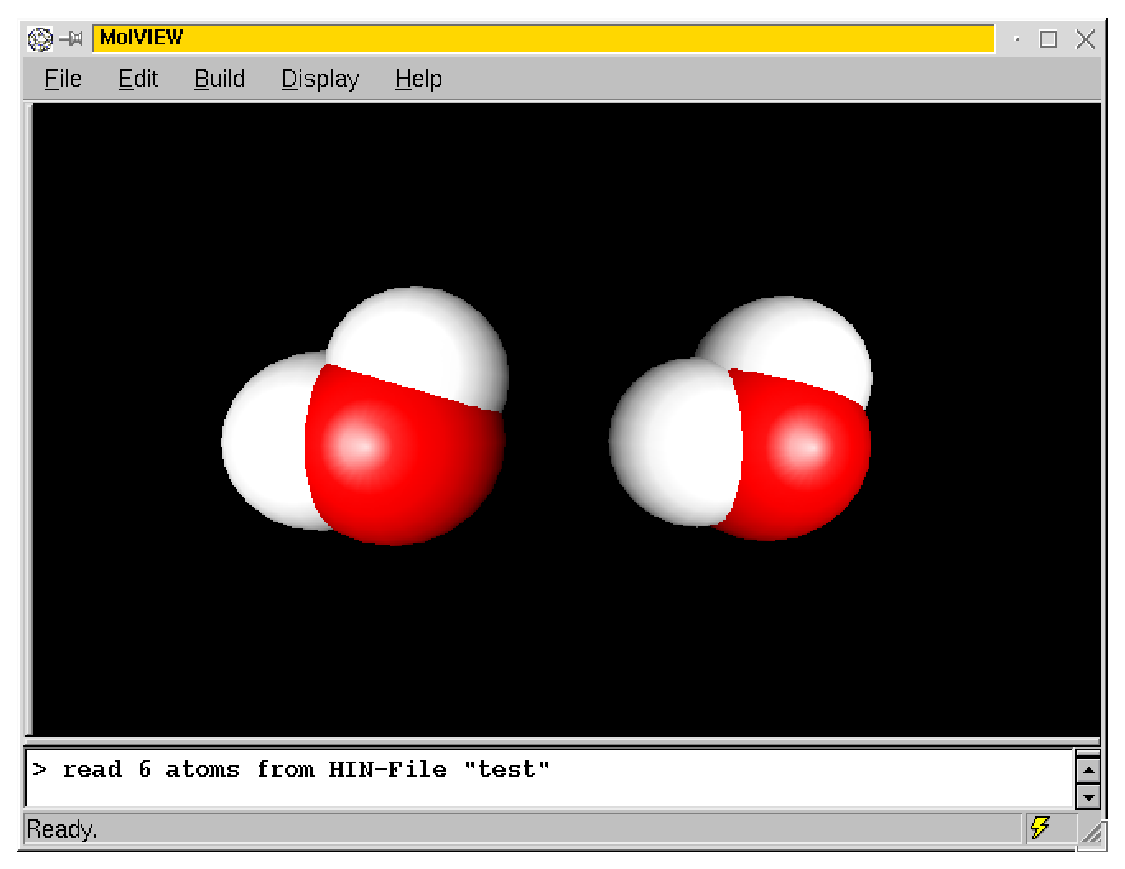
\includegraphics[width=\textwidth]{tut1_screenshot}
	\caption{Screenshot of BALLView showing the result of the first example
					 ({\tt tutorial1.C})}
	\label{fig:tut1-screenshot}
\end{figure}
\noindent
We can now manipulate the two water molecules simultaneously. For example a
further application of the translation processor to the system would apply
the translation to both molecules.
But now we would like to have a look at what we built. So we might write our
system to a file and inspect it with a molecule viewer (\eg BALLView).
BALL supports a variety of file formats. For example we could write the system
to a HyperChem HIN file~\cite{HyperChem}:
\begin{lstlisting}{}
	HINFile outfile("water.hin", File::OUT);
	outfile << S;
	outfile.close();
\end{lstlisting}
\noindent
These three lines of code create a \class{HINFile} object which is used to
read and write HyperChem files. The first line opens a file named {\tt
water.hin} for output ({\tt File::OUT}; if the second argument is omitted the
file is opened for reading only).
The second line uses the stream operator {\tt <<} to write the contents
of system {\tt S} to this file. The file is closed in the third line.

% ????? [anker]
% The following is not true. If we use a pointer here, then it's OK, but
% with a System it simply doesn't work. What do we want here? I'd prefer a
% Sytsem instead of a System*.

% Finally, we have to delete all the objects we created. This is very simple:
% 
% \begin{lstlisting}{}
% 	delete S;
% \end{lstlisting}

\noindent 
As all molecules and atoms we created are inside the system, they are deleted
automatically as soon as the system is deleted.

If this short program is run it creates the following output:

\begin{lstlisting}[frameround=]{}
	# of atoms in water: 3
	# of bonds of oxygen: 2
	# of bonds of hydrogen1: 1
	# of bonds of hydrogen2: 1
	bond distance: 0.95
\end{lstlisting}

\noindent
It also creates a file named {\tt water.hin} which contains the two water
molecules. Fig.~\ref{fig:tut1-screenshot} shows the contents of this file
in the BALLView viewer.

To compile this small example, we still have to include a few header files.
The complete file is shown in Listing~\ref{lst:tutorial1} on
page~\pageref{lst:tutorial1} and can be found in \mbox{{\tt
BALL/source/TUTORIAL/tutorial1.C}}.

First, we have to include \file{iostream} as we use {\tt cout} and {\tt endl}
to print some text. Then, we have to include the headers for the BALL kernel
classes \class{Atom}, \class{Bond}, \class{Molecule}, \class{System}, and
\class{PTE}. The headers for the HyperChem file support are found in the
directory \directory{BALL/FORMAT} and the headers for the
\class{TranslationProcessor} class are found in
{\tt BALL/STRUCTURE/geometricProperties.h}.

As all BALL classes are hidden in the \namespace{BALL} namespace, we have to
give access to this namespace with the command 
\begin{lstlisting}{}
	using namespace BALL;
\end{lstlisting}
Similarly, we also use the namespace \namespace{std} which contains {\tt cout}
and {\tt endl}.

If you have BALL installed, you might now try to compile this example. Simply
change to the directory \directory{BALL/source/TUTORIAL} which contains all
the examples from this tutorial and type 
\begin{lstlisting}[frameround=]{}
	make tutorial1
	./tutorial
\end{lstlisting}
This should build and execute the example. Please remember to set the
environment variable {\tt LD\_LIBRARY\_PATH} to the directory where your
libraries are installed.

After the successful execution of the example, a file named {\tt water.hin}
should appear in the current directory. This file contains the two water
molecules. You might inspect it with the molecule viewer BALLView.
Fig.~\ref{fig:tut1-screenshot} shows a screenshot of BALLView displaying the two
water molecules.

\newpage
\begin{lstlisting}[captionpos=t,caption={The complete source code of the first example.}\label{lst:tutorial1}]{}
// tutorial example 1
// ------------------
// build two water molecules and write them to a file

// needed for cout
#include <iostream>

// the BALL kernel classes
#include <BALL/KERNEL/atom.h>
#include <BALL/KERNEL/bond.h>
#include <BALL/KERNEL/molecule.h>
#include <BALL/KERNEL/system.h>
#include <BALL/KERNEL/PTE.h>

// reading and writing of HyperChem files
#include <BALL/FORMAT/HINFile.h>

// the TranslationProcessor
#include <BALL/STRUCTURE/geometricTransformations.h>

// we use the BALL namespace and the std namespace
using namespace BALL;
using namespace std;

int main()
{
	// we create a new atom called oxygen
	// and set its element to oxygen (PTE[Element::O])
	Atom* oxygen = new Atom;
	oxygen->setElement(PTE[Element::O]);

	// now we create two hydrogen atoms...
	Atom* hydrogen1 = new Atom;
	Atom* hydrogen2 = new Atom;
	hydrogen1->setElement(PTE[Element::H]);
	hydrogen2->setElement(PTE[Element::H]);

	// ...and move them to approximately correct positions
 	hydrogen1->setPosition(Vector3(-0.95, 0.00, 0.0));
 	hydrogen2->setPosition(Vector3( 0.25, 0.87, 0.0));

	// We create our water molecule...
	Molecule* water = new Molecule;

	// ...and insert the three atoms into the molecule.
	water->insert(*oxygen);
	water->insert(*hydrogen1);
	water->insert(*hydrogen2);

	// Then we build the two O-H bonds
	oxygen->createBond(*hydrogen1);
	oxygen->createBond(*hydrogen2);

	// Some statistics: Molecule::countAtoms() 
	// returns the number of atoms, Atom::countBonds() 
	// the number of bonds the atom shares
	cout << "# of atoms in water: " 
			 << water->countAtoms() << endl;
	cout << "# of bonds in oxygen: " 
			 << oxygen->countBonds() << endl;
	cout << "# of bonds of hydrogen1: " 
			 << hydrogen1->countBonds() << endl;
	cout << "# of bonds of hydrogen2: " 
			 << hydrogen2->countBonds() << endl;

	// bond_vector is a vector and is set to the
	// difference of atom positions of oxygen and hydrogen1
	Vector3 bond_vector = oxygen->getPosition() 
											- hydrogen1->getPosition();

	// Vector3::getLength: the length of the vector
	cout << "bond distance: " 
			 << bond_vector.getLength() << endl;

	// Now we copy our molecule using a copy constructor.
	Molecule* water2 = new Molecule(*water);

	// A translation processor moves the second molecule
	// 5 Angstrom along the x axis
	TranslationProcessor translation(Vector3(5, 0, 0));
	water2->apply(translation);

	// We insert our two molecules into a system
	System* S = new System;
	S->insert(*water);
	S->insert(*water2);

	// and write this system to a HyperChem file
	HINFile outfile("water.hin", File::OUT);
	outfile << *S;
	outfile.close();

	// We delete the system. This also deletes 
	// the molecules and the atoms therein
	delete S;
}
\end{lstlisting}
